The shuffled complex evolution is a population
based evolutionary optimization algorithm that regards a natural 
evolution happening simultaneously in $N$ independent communities (or complexes).

Initialy $N*M$ individuals are randomly taken from the feasible solution space and
sorted according to their fitness.
Subsequently a shuffling process places the \nth{1} in the first complex,
the \nth{2} in second complex, individual N\ts{th} goes to N\ts{th} complex,
individual $M+1$ goes back to the first complex, etc.
\begin{center}
\noindent\begin{tabular}{@{\hspace{0.0em}}c@{\hspace{1.0em}}c@{\hspace{0.0em}}}
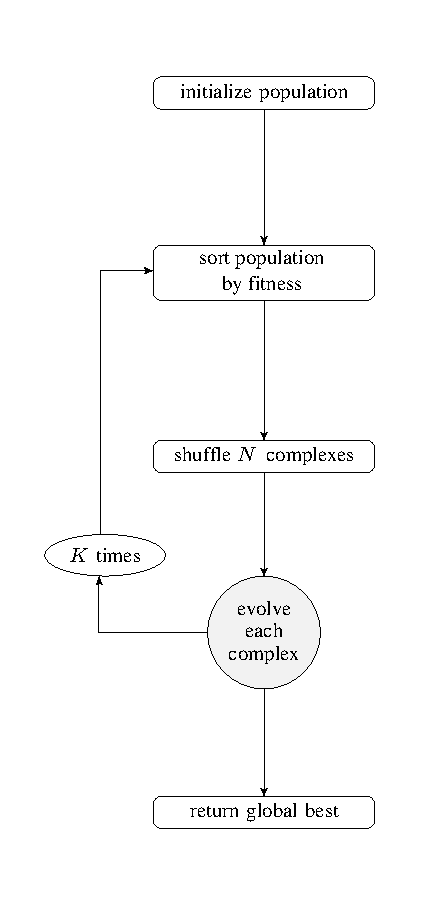
\includegraphics[width=0.46\linewidth]{imgs/flow1a} &
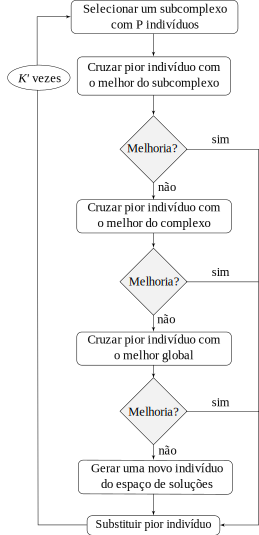
\includegraphics[width=0.46\linewidth]{imgs/flow2} 
\end{tabular}
\end{center}
\nocite{duan1992effective}
The next step after shuffling the complexes is to evolve each complex through
a given fixed amount of $K'$ steps:
the individuals in each complex is sorted by descending order of fitness quality.
In each step a subcomplex of $P$ individuals is selected from the
complex, prioritizing individuals with better fitness.

Then the worst individual from the subcomplex is identified to
be replaced by a new solution generated by its crossing 
with best individual of the subcomplex.
If the new solution has not improved, the best individual
of the complex is considered for crossing and latter the best individual
of whole population.
If all the crossing steps couldn't improve the worst solution,
it is replaced by a new random solution.
